\chapter{Overview e progettazione di sistema}
\label{chap:overview e progettazione di sistema}
In questo capitolo viene discusso lo scopo del progetto e le scelte progettuali adottate. Verranno toccati i principali problemi incontrati durante il lavoro e le loro risoluzioni. Infine, sarà descritta l'architettura del software con approfondimenti sui principali componenti.

\section{Scopo del progetto}
\label{sec:scopo del progetto}
Lo scopo principale del lavoro di tesi è quello di creare un sistema distribuito che permetta la visualizzazione real time, la storicizzazione e l'analisi delle transazioni  provenienti dalla blockchain di bitcoin. L'obiettivo principale è quello di riuscire a creare un sistema che gestisca grandi quantità di dati in un ambiente distribuito, garantendo affidabilità e consistenza dei dati anche in caso di guasti.
\\La prima grande sfida, quindi è stata quella di trovare un framework o un tool che permettesse di programmare su di un sistema distribuito, senza complicarci la vita. Facendo ricerche sul web la tecnologia che più si accostava meglio al mio problema è stata Apache Spark [\ref{sec:spark}]. Questo strumento riesce a garantire a pieno i vincoli che ci siamo imposti. Risolto il problema infrastrutturale si è proceduto all'analisi dei singoli sottoproblemi. 
\\L'applicazione fa uso dei blocchi grezzi da bitcoin, per testare il carico di lavoro sul sistema, per questo si è preferito utilizzare il software nativo del progetto Bitcoin: Bitcoind [\ref{sec:bitcoind}]. Bitcoind è un demone che invia blocchi o transazioni (a seconda di come lo si imposta) su di una coda di tipo publisher-subscriber tramite protocollo ZeroMQ [\ref{sec:ZMQ}]. Per raggiungere il nostro scopo, e quindi leggere i blocchi, è stato implementato in Spark un connettore che permette di leggere i dati real time dalla coda.
\\Ottenuti i blocchi dalla coda, il problema si è spostato sul conservare i dati ottenuti in modo da poterli processare ed analizzare. Fortunatamente, Spark offre una nativa collaborazione con il FileSystem distribuito Hadoop [\ref{sec:hadoop HDFS}], permettendomi di tenerli salvati su una memoria di massa.
\\Oltre ad Hadoop, i dati sono stati immagazzinati in Neo4j [\ref{sec:neo4j}]. Un database NoSQL che permette il salvataggio dei dati sottoforma di grafo, cosi da poter gestire facilmente i collegamenti tra le varie transazioni.
\\L'ultimo step, è stato quello di fare analisi delle transazioni, trovando i nodi con il maggior PageRank [\ref{sec:graphx (PageRank)}]. Anche in questo caso Spark è venuto in contro grazie al modulo GraphX, contenuto nel framework, il quale contiene algoritmi (come il PageRank) già sviluppati per l'analisi sui grafi.  
\\Una volta che il sistema distribuito è completo, non resta che mostrare i risultati ottenuti. Le scelte nel campo del front-end sono migliaia ma per semplicità ed una forte attitudine ai sistemi real-time si è preferito usare NodeJS [\ref{sec:nodejs}]. NodeJS ha infatti dei moduli che permettono l'accesso a Kafka, il tramite tra la parte di back-end e front-end. Inoltre, con NodeJS è stata costruita l'interfaccia grafica sottoforma di webapp, cosi da consentire gli utenti di visualizzare lo stato delle transazioni, i valori del PageRank e le transazioni che arrivano in real time.


\section{Architettura  del progetto}
\label{sec:architettura del progetto}

\subsection{Bitcoind}
\label{sec:bitcoind}
Bitcoind è un software che implementa il protocollo Bitcoin per l'utilizzo delle remote procedure call(RPC). Esso è anche il secondo client Bitcoin nella storia del network.\cite{wiki:bitcoind}.
Questo programma è la fonte dei dati per l'applicazione, difatti invia i blocchi  


\subsubsection{ZMQ}
\label{sec:ZMQ}

\subsection{Apache Spark}
\label{sec:spark}
Apache Spark è un framework di calcolo del cluster per l'elaborazione di dati su larga scala, progettato e implementato nel 2010 da un gruppo di ricercatori dell’Università di Berkeley a San Francisco \cite{spark:hadoop}. Questo progetto nasce dall'esigenza di migliorare le prestazioni dei sistemi distribuiti “MapReduce”. Per questo si sviluppa il concetto di Resilient Distributed Dataset (RDD), che è la teoria alla base del sistema Spark. Un RDD rappresenta un set di dati che è suddiviso in partizioni (Una tabella chiave-valore suddivisa in tante sotto-tabelle o un file diviso in tanti segmenti). Un RDD ha la proprietà di essere immutabile, cioè una volta creato non può essere cambiato se non creandone un altro. La creazione di un RDD avviene a partire dai dati su disco (presi da HDFS) o da altre fonti di dati. Una volta creato, un RDD può restare in memoria oppure può essere materializzato su disco. Ogni RDD è descritto da un set completo di metadati che consentono la ricostruzione di una delle sue partizioni in caso di fault. Spark nasce come un sistema per creare e gestire job di analisi basati su trasformazioni di RDD. Dato che gli RDD nascono e vivono in memoria, l’esecuzione di lavori iterativi, o che trasformano più volte un set di dati, sono immensamente più rapide di una sequenza di MapReduce; questo perchè il disco non viene mai (o quasi mai) impiegato nell’elaborazione.
\\Come detto in precedenza, Spark non utilizza MapReduce come motore di esecuzione; invece, utilizza il proprio runtime distribuito (DAG) per l’esecuzione di jobs su un cluster. Quando viene invocata un’azione su un RDD, viene creato un “job”. Un Directed Acyclic Graph o DAG è un grafo aciclico in cui ogni nodo è una partizione di RDD e ogni vertice è una trasformazione. A differenza di MapReduce, il motore DAG di Spark può processare pipeline arbitrarie di operatori e tradurle in un unico “job” per l'utente.
\\Spark, infine, sta dimostrando di essere una buona piattaforma su cui costruire strumenti di analisi, infatti ha moduli per il Machine learning (MLlib), Elaborazione grafica (GraphX), Elaborazione di stream (Spark Streaming) ed SQL (Spark SQL) \cite{spark:hadoop}.
\begin{figure}[H]
	\centering
	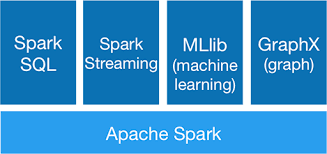
\includegraphics[width=\textwidth]{images/spark.png}
	\caption{Infrastruttura Spark.}
	\label{fig:sparkOverview}
\end{figure}
Nel sistema distribuito, poichè c'è l'esigenza di recuperare i dati in real time dalla coda di bitcoind, viene utilizzato Spark Streaming. Questo modulo è un'estensione dell'API Spark di base che consente l'elaborazione streaming, scalabile, ad alto throughput e con tolleranza agli errori dei flussi di dati in tempo reale. I dati, che possono provenire da diverse fonti, sono elaborati utilizzando algoritmi complessi espressi con funzioni di alto livello come \textit{map}, \textit{reduce}, \textit{join} e \textit{window}. I dati processati, infine possono essere inviati a filesystem (Hadoop) o database (Neo4j) per il salvataggio oppure ad altri moduli di Spark, dediti all'analisi, tipo machine learning (MLlib) o graph processing (GraphX). 
\\Internamente, Spark Streaming riceve streams di dati di input e li divide in batch, che vengono quindi elaborati dal motore Spark per generare il flusso finale di risultati. Per consentire il facile utilizzo di questi dati, fornisce un'astrazione di alto livello chiamata stream discretizzato o DStream, che rappresenta un flusso continuo di dati. E' possibile creare Dstreams da flussi di dati di input da sorgenti come Kafka, Flume e Kinesis o applicando operazioni di alto livello su altri Dstreams \cite{spark:home-streaming}. Internamente, un Dstream è rappresentato come una sequenza di RDD sulla quale possono essere effettuate le operazioni descritte in precedenza.
\begin{figure}[H]
	\centering
	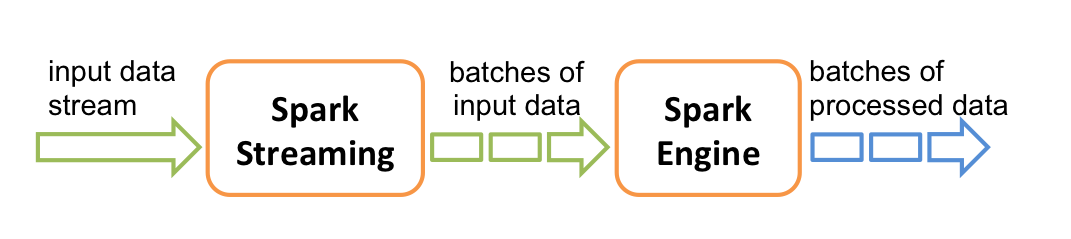
\includegraphics[width=\textwidth]{images/streamingSpark.png}
	\caption{Come vengono gestiti i dati in Spark Streaming.}
	\label{fig:streamingSpark}
\end{figure}
Nel sistema distribuito, per fare analisi dei dati provenienti dall'elaborazione di Spark, è stato scelto il modulo interno GraphX.
\\GraphX è un nuovo componetene di Apache Spark per grafi ed il calcolo parallelo (PageRank) su di essi. Estende gli RDD di spark introducendo gli Resilient Distribuited Property Graph, oggetti simili a grafi che permettono l'inserimento di proprietà per vertici e archi, rendendo facilitata l'implementazione. Inoltre, per aiutare nell'analisi, espone un insieme di operatori fondamentali (sottografo, joinVertices e aggregateMessages) come variante ottimizzata dell'API Pregel. In più, Graphx include una crescente collezione di algoritmi e costrutti per grafi per semplificare le attività di analisi \cite{spark:graphx}. Attualmente le sue API sono scritte in Scala, Java e Python.
\begin{figure}[H]
	\centering
	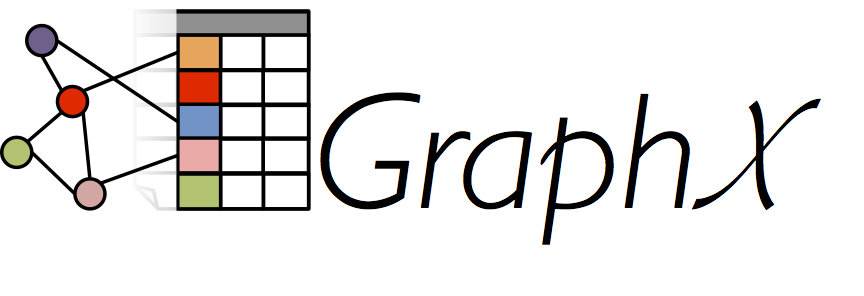
\includegraphics[width=\textwidth]{images/graphxLogo.png}
	\caption{Logo GraphX.}
	\label{fig:graphxLogo}
\end{figure}
GraphX, come detto in precedenza, gestisce i dati in memoria come se fossero grafi. Infatti, utilizza archi e vertici che hanno delle proprietà  connesse. Ogni vertice possiede un identificativo univoco a 64bit (VertexID), mentre, allo stesso modo, gli archi contengono gli identificativi di origine e partenza. Queste proprietà sono definite e tenuti in memoria come oggetti e di conseguenza con metodi creati ad-hoc per gestirli.  


\subsection{Hadoop HDFS}
\label{sec:hadoop HDFS}

\subsection{Neo4j}
\label{sec:neo4j}



\subsection{Zookeeper}
\label{sec:zookeeper}

\subsubsection{Kafka}
\label{sec:kafka}
\section{WebApp}
\label{sec:webapp}
Una applicazione web è una applicazione client/server per un ambiente stateless, cioè senza memoria, che utilizza le tecnologie internet. Con il termine Webapp si descrive un'applicazione accessibile via web per mezzo di una network, come ad esempio una Intranet o attraverso la rete Internet. Pertanto, saper programmare per il web significa conoscere i diversi meccanismi e strumenti per conservare o passare i dati, detti parametri, tra le diverse pagine dell'applicazione web. In pratica una Web-application, è un programma che non necessita di essere installato nel computer in quanto esso si rende disponibile su un server in rete e può essere fatto funzionare attraverso un normale Web browser (es. Google Chrome, Mozilla Firefox, Opera, ecc.). I client, dopo aver instaurato una connessione con il server, invia la richiesta per un servizio; il server dopo aver elaborato i dati necessari rende disponibile al client il servizio richiesto. A differenza dei siti web statici (HTML), l'applicazione web viene realizzata con una o più tecnologie (Javascript, Ajax, Servlet, Database ecc.) che permettono la creazione di un sito dinamico, cioè di un sito nel quale il contenuto delle pagine varia durante l'interazione.
\\Le applicazioni Web si pongono come valida alternativa alle tradizionali applicazioni Client/Server per vari motivi:
\begin{itemize}
\item \textit{Facilità di distribuzione e aggiornamento}: un'applicazione Web risiede interamente sul server, per cui la sua pubblicazione coincide con la distribuzione e l'aggiornamento ed è automaticamente disponibile a tutti gli utenti.
\item \textit{Accesso multi-piattaforma}: l'accesso all'applicazione è indipendente dall'hardware e dal sistema operativo utilizzato dagli utenti;
\item \textit{Riduzione del costo di gestione}: l'uso di Internet come infrastruttura per un'applicazione Web riduce notevolmente sia i costi di connettività che i costi di gestione dei client;
\item \textit{Scalabilità}: un'applicazione Web ben progettata può crescere insieme alle esigenze dell'azienda senza particolari problemi;
\end{itemize}
Per poter mostrare l'elaborazione di Spark nel sistema distribuito, si è preferito utilizzare una webapp per i motivi sopra citati. Questa applicazione web fa uso di tecnologie di ultima generazione quali NodeJs ed HTML5. Questo la rende fruibile a tutti gli utenti provvisti di Pc, Tablet o Smartphone con un browser installato. Nel seguente capito dunque vengono messi in luce i principali componenti che compongono la webapp, mostrando i punti forti di ogni tecnologia.
\begin{figure}[H]
	\centering
	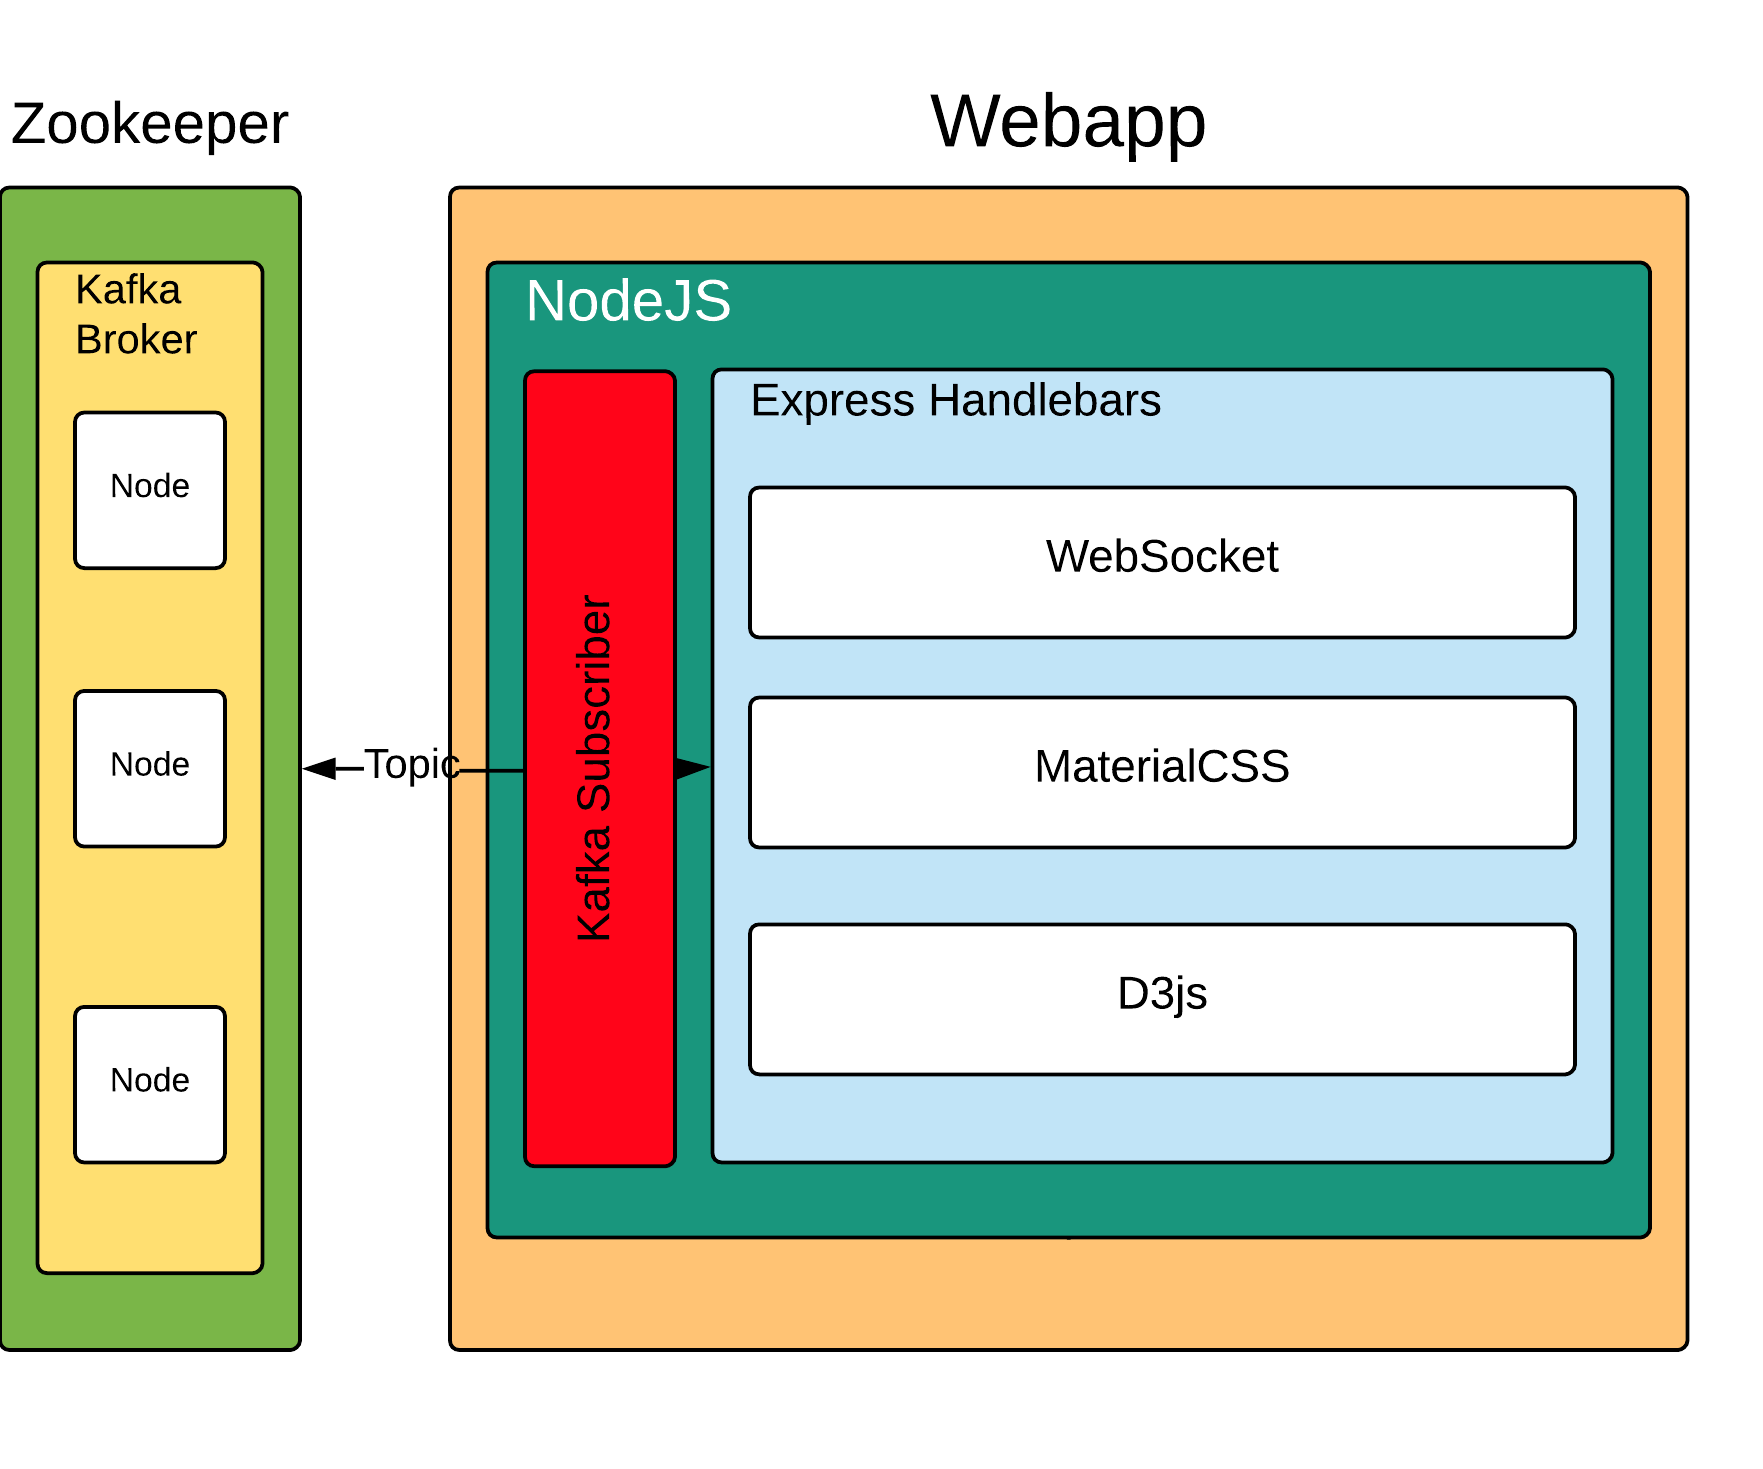
\includegraphics[width=\textwidth]{images/webApp.png}
	\caption{Architettura in dettaglio della webapp.}
	\label{fig:webAppArchitetture}
\end{figure}